    \chapter{User guide}

\section{Registration}
\label{sec:registration}

\subsection{Step 1}
The reimbursement-tool is connected to the UZH-IFI LDAP server. This allows employees of the IFI department to use their existing login-credentials provided by the University of Zurich to login to the reimbursement-tool.\newline
After the initial login a user needs to pass a two-step registration process. On figure \ref{fig:registration-step01} the user needs to input two values:
\begin{itemize}
    \item UZH personnel number is the employee number, written on the employment card. It is of the form \textit{01-123-456}. Enter the number without the leading 0 and hyphens; i.e. \textit{123456}.
    \item UZH phone number is the personnel phone number of the employee. Please enter it in the form \textit{0441234567}.
\end{itemize}\newpage


\begin{figure}[H]
    \centering
    \fbox{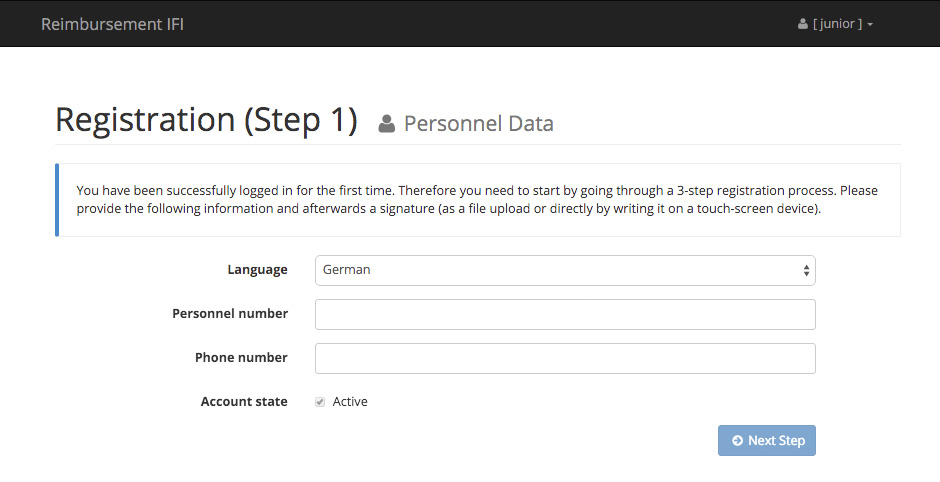
\includegraphics[width=0.80\textwidth]{registration-step01}}
    \caption{Registration step one: Capture personnel data}
    \label{fig:registration-step01}
\end{figure}

\subsection{Step 2}
On figure \ref{fig:registration-step02} the user needs to add his handwritten signature either by uploading an image or capture it using a third party touchscreen device, like a smart phone. This signature is required to sign the generated Pdf document containing all \textit{Receipts}.

\begin{figure}[H]
    \centering
    \fbox{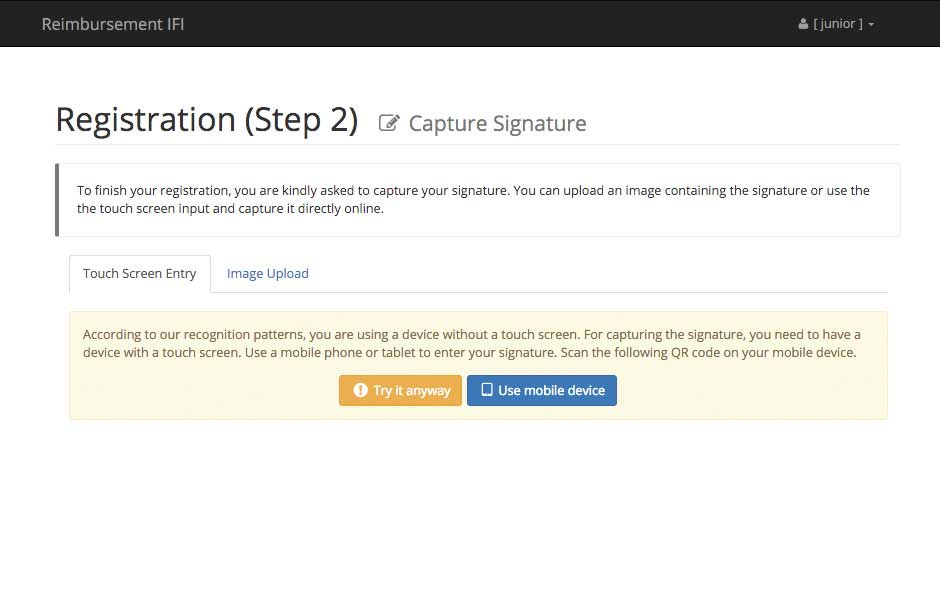
\includegraphics[width=0.80\textwidth]{registration-step02}}
    \caption{Registration step two: Capture signature}
    \label{fig:registration-step02}
\end{figure}

After completing the registration process, these captured information and signature can always be edited by navigation to the \textbf{Settings} on the navigation bar.
\clearpage

\section{Expenses}

An \textit{Expense} is an entity captured by an \textit{Registered user}. Every \textit{Expense} is defined by an \textbf{accounting description} that will be visual in SAP. An \textit{Expense} consists of 1 to 15 \textit{Receipts}.

The \textit{Registered user} has to create an \textit{Expense}, add \textit{Receipts} to it and assign it to his \textit{Manager}. The \textit{Manager} will check the \textit{Expense} for correctness, add the corresponding projects and assign it to the \textit{Finance administration} if the \textit{Expense} is correct. For a detailed description of the process refer to section \ref{sec:process}.

\subsection{Create Expense}

To create an \textit{Expense}, the user needs to navigate to the \textbf{Dashboard} and click on the button \textbf{Create new Expense}. A modal-window will appear to enter an SAP description.\newline Once the \textit{SAP description} is entered correctly and the user clicked \textbf{Next} an empty \textit{Expense} will be created. The user can start with adding \textit{Receipts} (see figure \ref{fig:expensesitems-overview}).

\begin{figure}[H]
    \centering
    \fbox{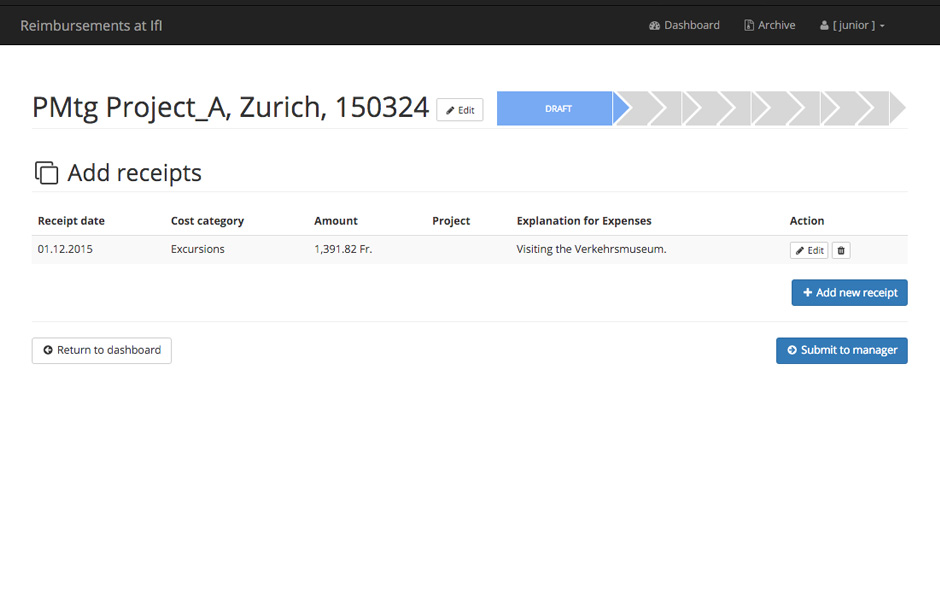
\includegraphics[width=0.80\textwidth]{expensesItems-overview}}
    \caption{Expense-View: Overview}
    \label{fig:expensesitems-overview}
\end{figure}

On the top left-hand side the \textit{SAP description} is added. The small button on the right can be used for editing. On the top right-hand side the current process step and the unprocessed steps of the \textit{Expense} are visualized. This process bar always indicates the state the \textit{Expense} is currently at.\newline
Further the user can add, edit and remove \textit{Receipts}. To add a new \textit{Receipt} the user needs to click on the button \textbf{Add new Receipt}. See Section \ref{sec:addreceipt} for details.\newline
Existing \textit{Receipts} can be edited and removed by clicking on the respective buttons at the Receipts-list.


\subsection{Receipt}
\label{sec:addreceipt}
By adding a new \textit{Receipt} or editing an existing one, the user needs to fill out the following mandatory information:
\begin{itemize}
    \item \textbf{Receipt date} will further be used to calculate the correct exchange rate if a foreign currency is selected.
    \item \textbf{Cost category} selected based on a pre-defined list of available cost categories.
    \item Original and calculated amount based on the exchange rate.
    \item The \textbf{project assignment} is added by a user with role \textit{Manager} or \textit{Department manager}.
    \item A short \textbf{explanation} that describes the purpose of the \textit{Receipt}.
    \item \textbf{Receipt attachment} used for verification purpose of the entered \textit{Receipt} data.
\end{itemize}

See figure \ref{fig:expenses-add01} for details.


\begin{figure}[H]
    \centering
    \fbox{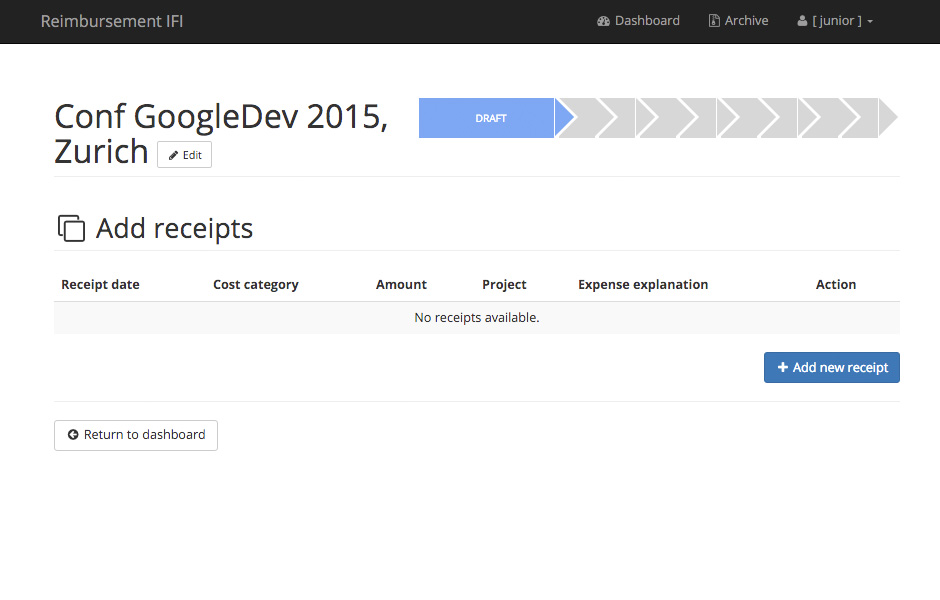
\includegraphics[width=0.80\textwidth]{expenses-add01}}
    \caption{Expense: Add new receipt}
    \label{fig:expenses-add01}
\end{figure}

\subsection{Assign Expense to Professor}
If all \textit{Receipts} are captured, the \textit{Expense} will be assigned to the \textit{Manager} in charge. Once the assignment is processed, the \textit{Expense} cannot be edited by the user anymore. To assign an \textit{Expense} to the \textit{Manager}, click on the \textbf{Submit to Manager} button.

\subsection{States}
\label{sec:states}
Every \textit{Expense} is always in one of the following states during the process:

\begin{itemize}
    \item \textbf{Draft} state occurs if the \textit{Expense} is created and yet has not been assigned to a \textit{Manager}.
    
    \item \textbf{To be assigned} state occurs if the \textit{Expense} is submitted to the \textit{Manager} but has not been assigned to a specific \textit{Manager}.
    
    \item \textbf{Assigned to Manager} state occurs if the \textit{Expense} is submitted to the \textit{Manager} and has been assigned to a specific \textit{Manager}.
    
    \item \textbf{Assigned to Finance Admin} state occurs if the \textit{Expense} is submitted to the \textit{Manager} and has been assigned to a specific \textit{Finance admin}.
    
    \item \textbf{Rejected} state occurs if the created \textit{Expense} is not accepted by the \textit{Manager}, \textit{Department manager} or \textit{Finance management}. In \textbf{Rejected} status the \textit{Expense} will be reassigned to the user who created it.
    
    \item \textbf{Signed} state occurs if the \textit{Expense} has been signed by all participants; \textit{Registered user}, \textit{Manager} or \textit{Department manager} and \textit{Finance management}. There exist sub states that occur if the \textit{Expense} is in the process of being signed by all participants:
        \begin{itemize}
            \item \textbf{To be signed by \textit{User}} occurs if the \textit{Expense} needs to be signed by the \textit{User}.
            \item \textbf{To be signed by \textit{Manager}} occurs if the \textit{Expense} needs to be signed by the \textit{Manager}.
            \item \textbf{To be signed by \textit{Finance admin}} occurs if the \textit{Expense} needs to be signed by the \textit{Finance admin}.
        \end{itemize}
    
    \item \textbf{Printed} state occurs if the \textit{Expense} and all its \textit{Receipts} are successfully converted into a digital document.
    
\end{itemize}

\subsection{Sign document}
\label{sec:signing}
The signing is needed for the generation of the Pdf that contains all of the captures \textit{Expenses} and \textit{Receipts}. This Pdf uses the signatures of the respective \textit{User}, \textit{Manager} and \textit{Finance admin} to proof their acceptance of the captures \textit{Expenses} and \textit{Receipts}. During the signing process the user will be prompted to select his preferred signing method (see figure 3.5). The two different types available will be explained in detail:
    \begin{itemize}
        \item A \textbf{Digital signature} ensure the authenticity of the signer. Any changes made to the document after it has been signed will invalidate the signature. To use the \textit{Digital signature} the user has to provide his private key to successfully sign the document.
        \item \textbf{Electronic signature} does not ensure the authenticity of the signer. Anyone can theoretically make changes on the document after it has been signed without the signature become invalid. To use it, the user only has to add his handwritten signature.
    \end{itemize}
    
\begin{figure}[H]
    \centering
    \fbox{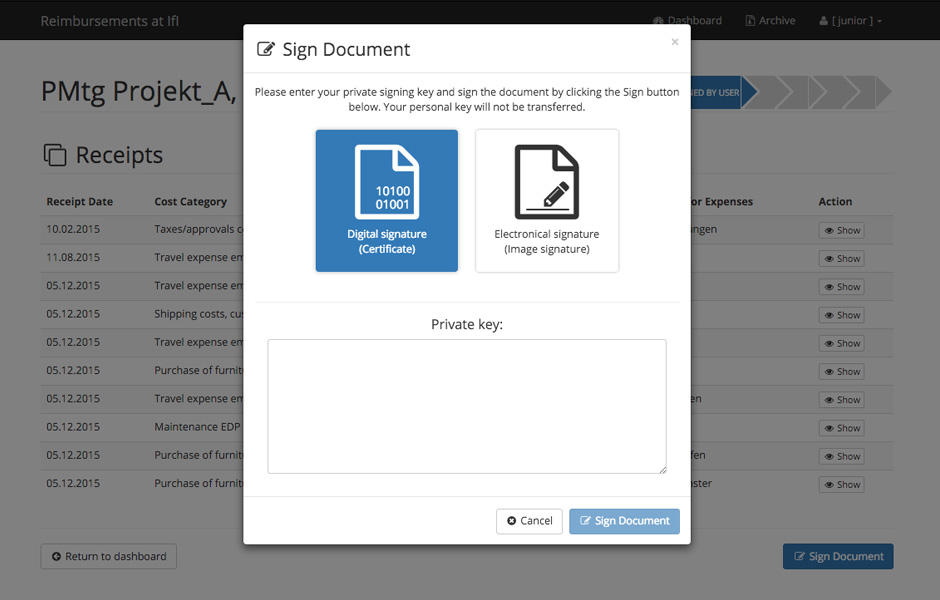
\includegraphics[width=0.80\textwidth]{expenses-sign}}
    \caption{Expense: Sign document}
    \label{fig:expense-sign}
\end{figure}

Please note, that if a signing method has been selected all subsequent signers, like \textit{Manager} and \textit{Finance management} have to apply the same method.


\section{User}

Every user that exists in the LDAP of the University of Zurich is capable to login to the system. He can use the same user name and password that he uses for the other University of Zurich services for login. See Section \ref{sec:registration} for more details.

There exists different roles for users to login to the system. A user is allowed to have exactly one role out of the four defined. The roles are provided and synchronized with the LDAP-Server of the University of Zurich. The following roles exist in the system:

\begin{itemize}
    \item \textbf{Unregistered user} are users, who are authorized to login the reimbursement-tool but have not yet completed the registration process, see section \ref{sec:registration}.
    \item \textbf{Registered user / User} are authorized to create and edit \textit{Expenses} that they created. However, an \textit{Expense} cannot be edited once it has been assigned to a \textit{Manager}.
    
    \item \textbf{Manager / Professor} are authorized to reject, accept and edit \textit{Expenses}. A \textit{Manager} is also capable of creating \textit{Expenses} and editing them until it has been assigned. 
    
    \item \textbf{Department manager} has the same authorizations as the \textit{Manager}. If a \textit{Manager} is outreach his assignments will be forwarded to the \textit{Department manager}. There exist multiple \textit{Department manager}.
    
    \item \textbf{Finance management / Finance admin} is authorized to reject, accept and edit \textit{Expenses} once they have been accepted by a \textit{Manager} or \textit{Department managers}. Furthermore they can manage the available cost categories.
    
    \item \textbf{Head of institute} has the same authorizations as the \textit{Manager}. In contrast to the \textbf{Department manager} there exists only one \textit{Head of institute}.
\end{itemize}

\section{Guest view}
The guest view allows users to retrieve \textit{Expenses} without the need of valid login-credentials for the reimbursement-tool. They can open the guest view using a special URL, provided on every printed \textit{Expense} document. The URL is located on the second page in form of a QR-Code and an URL. So that the user can either scan the QR-Code or typewrite the URL in a browser window and he'll get access to the respective \textit{Expense}.

\section{Cost categories}

The existing cost categories of the reimbursement-tool can be edited and deactivated by the \textit{Finance management}. Furthermore a new cost category can be created by providing the German and English translation for it. See figure \ref{fig:admin-costcategories}.

\begin{figure}[H]
    \centering
    \fbox{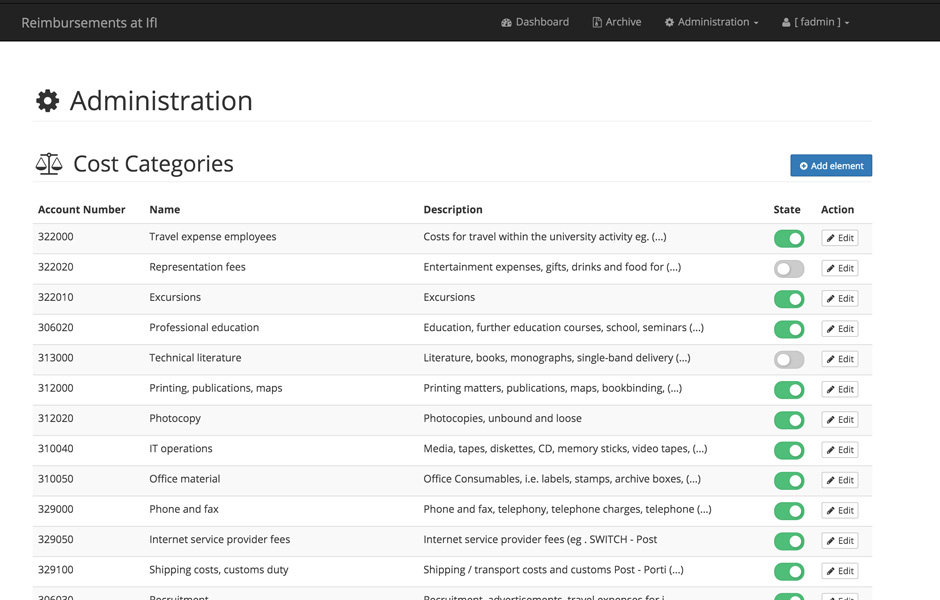
\includegraphics[width=0.80\textwidth]{admin-costcategories}}
    \caption{Administration: Cost categories}
    \label{fig:admin-costcategories}
\end{figure}

\section{Retrieve Expenses}
\subsection{Search for Expenses}

For the \textit{Finance management} a sophisticated search interface for \textit{Expenses} exist; the \textit{Admin Pool Search}. See figure \ref{fig:admin-search}. The search results will be limited by the following values:

\begin{itemize}
    \item Specify the date range the \textit{Expense} has been created.
    \item Last name of the \textit{Expense} applicant.
    \item The permission / role of the applicant.
    \item The current state of the \textit{Expense}.
    \item Based on the selected cost category of the \textit{Receipt}.
    \item The accounting description (similar to the SAP description).
\end{itemize}

\begin{figure}[H]
    \centering
    \fbox{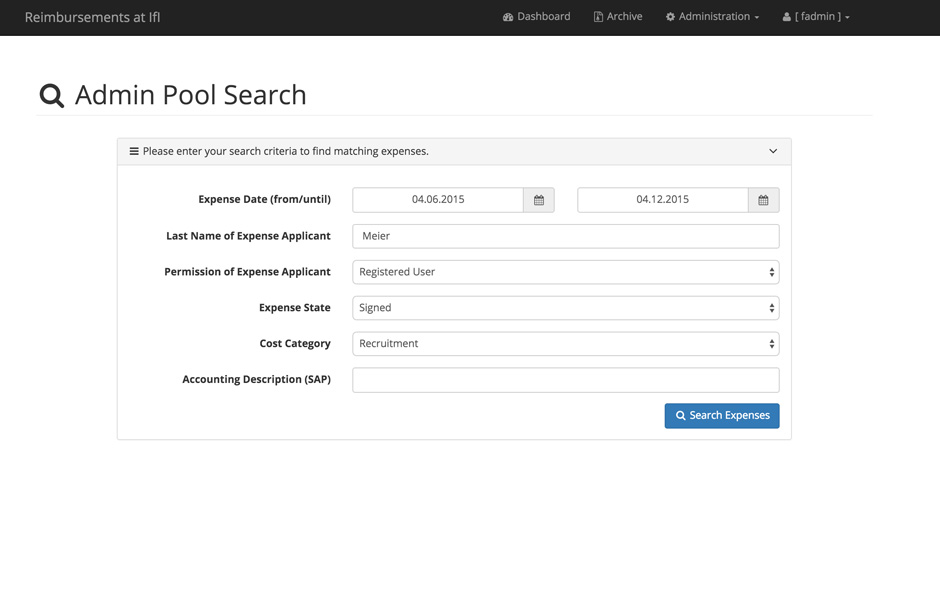
\includegraphics[width=0.80\textwidth]{admin-search}}
    \caption{Administration: Search for \textit{Expenses}}
    \label{fig:admin-search}
\end{figure}

The \textit{Finance admin} is authorized to override the following \textit{Expense} states:
\begin{itemize}
\item \textbf{Reassign}: If the \textit{Expense} is in \textit{Printed} state, it can be reassigned to the \textit{Finance admin}.
\item \textbf{Reset}: During the 1. Iteration (see section \ref{sec:process}) the \textit{Expense} can be reset to send it back to the creator. The \textit{Expense} state will change to \textit{Draft}. 
\end{itemize}

\subsection{Archive}
Besides the \textit{Admin Pool Search} there exists an archive interface for all users. The archive provides a list of all \textit{Expenses} in \textit{Printed} state that the current user has created.\newpage  

\section{Expense process}
\label{sec:process}

The entire process is basically divided into three iterations. The \textbf{1. iteration}; Expense creation, \textbf{2. iteration}; the Expense signing, the \textbf{3. iteration}; print and carry the documents to the finance administration of the University of Zurich.\newline 
Expense date, cost category, amount, explanation and attachment will be captured by the user to initiate the first iteration. As soon as the user is done with the capturing the Expense will be assigned to the \textit{Manager}. He reviews the Expense, adds the respective projects and assigns the Expense to the next instance for review; the \textit{Finance Management}. If they are satisfied the Expense moves into the second iteration; the signing. For more detailed information containing the signing refer to section \ref{sec:signing}.\newline

\begin{figure}[H]
    \centering
    \fbox{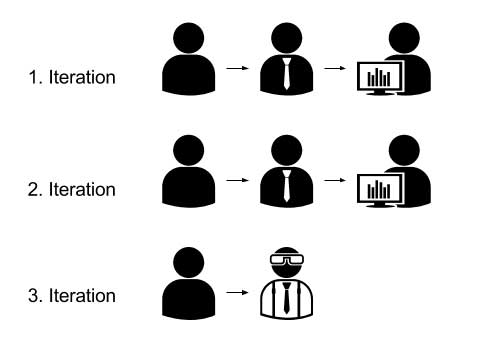
\includegraphics[width=0.80\textwidth]{expense-process}}
    \caption{Expense: Process of expense creation}
    \label{fig:expense-process}
\end{figure}

After the signing is completed by all instances. The \textit{Expense} will be available to print by its creator. As soon as all the documents are printed, they need to be carried to the respective \textit{Finance admin} for further processing. The \textit{Finance admin} will send all relevant documents to the finance adminstration of the University of Zurich. This action completes the process.   

